%  A simple AAU report template.
%  2015-05-08 v. 1.2.0
%  Copyright 2010-2015 by Jesper Kjær Nielsen <jkn@es.aau.dk>
%
%  This is free software: you can redistribute it and/or modify
%  it under the terms of the GNU General Public License as published by
%  the Free Software Foundation, either version 3 of the License, or
%  (at your option) any later version.
%
%  This is distributed in the hope that it will be useful,
%  but WITHOUT ANY WARRANTY; without even the implied warranty of
%  MERCHANTABILITY or FITNESS FOR A PARTICULAR PURPOSE.  See the
%  GNU General Public License for more details.
%
%  You can find the GNU General Public License at <http://www.gnu.org/licenses/>.
%
%  A simple AAU report template.
%  2015-05-08 v. 1.2.0
%  Copyright 2010-2015 by Jesper Kjær Nielsen <jkn@es.aau.dk>
%
%  This is free software: you can redistribute it and/or modify
%  it under the terms of the GNU General Public License as published by
%  the Free Software Foundation, either version 3 of the License, or
%  (at your option) any later version.
%
%  This is distributed in the hope that it will be useful,
%  but WITHOUT ANY WARRANTY; without even the implied warranty of
%  MERCHANTABILITY or FITNESS FOR A PARTICULAR PURPOSE.  See the
%  GNU General Public License for more details.
%
%  You can find the GNU General Public License at <http://www.gnu.org/licenses/>.
%
\documentclass[11pt,twoside,a4paper,openright]{report}
%%%%%%%%%%%%%%%%%%%%%%%%%%%%%%%%%%%%%%%%%%%%%%%%
% Language, Encoding and Fonts
% http://en.wikibooks.org/wiki/LaTeX/Internationalization
%%%%%%%%%%%%%%%%%%%%%%%%%%%%%%%%%%%%%%%%%%%%%%%%
% Select encoding of your inputs. Depends on
% your operating system and its default input
% encoding. Typically, you should use
%   Linux  : utf8 (most modern Linux distributions)
%            latin1 
%   Windows: ansinew
%            latin1 (works in most cases)
%   Mac    : applemac
% Notice that you can manually change the input
% encoding of your files by selecting "save as"
% an select the desired input encoding. 
\usepackage[utf8]{inputenc}
% Make latex understand and use the typographic
% rules of the language used in the document.
\usepackage[danish,english]{babel}
% Use the palatino font
\usepackage[sc]{mathpazo}
\linespread{1.05}         % Palatino needs more leading (space between lines)
% Choose the font encoding
\usepackage[T1]{fontenc}
%%%%%%%%%%%%%%%%%%%%%%%%%%%%%%%%%%%%%%%%%%%%%%%%
% Graphics and Tables
% http://en.wikibooks.org/wiki/LaTeX/Importing_Graphics
% http://en.wikibooks.org/wiki/LaTeX/Tables
% http://en.wikibooks.org/wiki/LaTeX/Colors
%%%%%%%%%%%%%%%%%%%%%%%%%%%%%%%%%%%%%%%%%%%%%%%%
% load a colour package
\usepackage{xcolor}
\definecolor{aaublue}{RGB}{33,26,82}% dark blue
% The standard graphics inclusion package
\usepackage{graphicx}
% Set up how figure and table captions are displayed
\usepackage{caption}
\captionsetup{%
  font=footnotesize,% set font size to footnotesize
  labelfont=bf % bold label (e.g., Figure 3.2) font
}
% Make the standard latex tables look so much better
\usepackage{array,booktabs}
% Enable the use of frames around, e.g., theorems
% The framed package is used in the example environment
\usepackage{framed}

%%%%%%%%%%%%%%%%%%%%%%%%%%%%%%%%%%%%%%%%%%%%%%%%
% Mathematics
% http://en.wikibooks.org/wiki/LaTeX/Mathematics
%%%%%%%%%%%%%%%%%%%%%%%%%%%%%%%%%%%%%%%%%%%%%%%%
% Defines new environments such as equation,
% align and split 
\usepackage{amsmath}
% Adds new math symbols
\usepackage{amssymb}
% Use theorems in your document
% The ntheorem package is also used for the example environment
% When using thmmarks, amsmath must be an option as well. Otherwise \eqref doesn't work anymore.
\usepackage[framed,amsmath,thmmarks]{ntheorem}

%%%%%%%%%%%%%%%%%%%%%%%%%%%%%%%%%%%%%%%%%%%%%%%%
% Page Layout
% http://en.wikibooks.org/wiki/LaTeX/Page_Layout
%%%%%%%%%%%%%%%%%%%%%%%%%%%%%%%%%%%%%%%%%%%%%%%%
% Change margins, papersize, etc of the document
\usepackage[
  inner=28mm,% left margin on an odd page
  outer=41mm,% right margin on an odd page
  ]{geometry}
% Modify how \chapter, \section, etc. look
% The titlesec package is very configureable
\usepackage{titlesec}
\titleformat{\chapter}[display]{\normalfont\huge\bfseries}{\chaptertitlename\ \thechapter}{20pt}{\Huge}
\titleformat*{\section}{\normalfont\Large\bfseries}
\titleformat*{\subsection}{\normalfont\large\bfseries}
\titleformat*{\subsubsection}{\normalfont\normalsize\bfseries}
%\titleformat*{\paragraph}{\normalfont\normalsize\bfseries}
%\titleformat*{\subparagraph}{\normalfont\normalsize\bfseries}

% Clear empty pages between chapters
\let\origdoublepage\cleardoublepage
\newcommand{\clearemptydoublepage}{%
  \clearpage
  {\pagestyle{empty}\origdoublepage}%
}
\let\cleardoublepage\clearemptydoublepage

% Change the headers and footers
\usepackage{fancyhdr}
\pagestyle{fancy}
\fancyhf{} %delete everything
\renewcommand{\headrulewidth}{0pt} %remove the horizontal line in the header
\fancyhead[RE]{\small\nouppercase\leftmark} %even page - chapter title
\fancyhead[LO]{\small\nouppercase\rightmark} %uneven page - section title
\fancyhead[LE,RO]{\thepage} %page number on all pages
% Do not stretch the content of a page. Instead,
% insert white space at the bottom of the page
\raggedbottom
% Enable arithmetics with length. Useful when
% typesetting the layout.
\usepackage{calc}

%%%%%%%%%%%%%%%%%%%%%%%%%%%%%%%%%%%%%%%%%%%%%%%%
% Bibliography
% http://en.wikibooks.org/wiki/LaTeX/Bibliography_Management
%%%%%%%%%%%%%%%%%%%%%%%%%%%%%%%%%%%%%%%%%%%%%%%%
\usepackage[backend=bibtex,
  bibencoding=utf8
  ]{biblatex}
\addbibresource{bib/mybib}

%%%%%%%%%%%%%%%%%%%%%%%%%%%%%%%%%%%%%%%%%%%%%%%%
% Misc
%%%%%%%%%%%%%%%%%%%%%%%%%%%%%%%%%%%%%%%%%%%%%%%%
% Add bibliography and index to the table of
% contents
\usepackage[nottoc]{tocbibind}
% Add the command \pageref{LastPage} which refers to the
% page number of the last page
\usepackage{lastpage}
% Add todo notes in the margin of the document
\usepackage[
%  disable, %turn off todonotes
  colorinlistoftodos, %enable a coloured square in the list of todos
  textwidth=\marginparwidth, %set the width of the todonotes
  textsize=scriptsize, %size of the text in the todonotes
  ]{todonotes}

%%%%%%%%%%%%%%%%%%%%%%%%%%%%%%%%%%%%%%%%%%%%%%%%
% Hyperlinks
% http://en.wikibooks.org/wiki/LaTeX/Hyperlinks
%%%%%%%%%%%%%%%%%%%%%%%%%%%%%%%%%%%%%%%%%%%%%%%%
% Enable hyperlinks and insert info into the pdf
% file. Hypperref should be loaded as one of the 
% last packages
\usepackage{hyperref}
\hypersetup{%
	pdfpagelabels=true,%
	plainpages=false,%
	pdfauthor={Author(s)},%
	pdftitle={Title},%
	pdfsubject={Subject},%
	bookmarksnumbered=true,%
	colorlinks=false,%
	citecolor=black,%
	filecolor=black,%
	linkcolor=black,% you should probably change this to black before printing
	urlcolor=black,%
	pdfstartview=FitH%
}
% package inclusion and set up of the document
% see, e.g., http://en.wikibooks.org/wiki/LaTeX/Formatting#Hyphenation
% for more information on word hyphenation
\hyphenation{ex-am-ple hy-phen-a-tion short}
\hyphenation{long la-tex}% 
%  A simple AAU report template.
%  2015-05-08 v. 1.2.0
%  Copyright 2010-2015 by Jesper Kjær Nielsen <jkn@es.aau.dk>
%
%  This is free software: you can redistribute it and/or modify
%  it under the terms of the GNU General Public License as published by
%  the Free Software Foundation, either version 3 of the License, or
%  (at your option) any later version.
%
%  This is distributed in the hope that it will be useful,
%  but WITHOUT ANY WARRANTY; without even the implied warranty of
%  MERCHANTABILITY or FITNESS FOR A PARTICULAR PURPOSE.  See the
%  GNU General Public License for more details.
%
%  You can find the GNU General Public License at <http://www.gnu.org/licenses/>.
%
%
%
% see, e.g., http://en.wikibooks.org/wiki/LaTeX/Customizing_LaTeX#New_commands
% for more information on how to create macros

%%%%%%%%%%%%%%%%%%%%%%%%%%%%%%%%%%%%%%%%%%%%%%%%
% Macros for the titlepage
%%%%%%%%%%%%%%%%%%%%%%%%%%%%%%%%%%%%%%%%%%%%%%%%
%Creates the aau titlepage
\newcommand{\aautitlepage}[3]{%
  {
    %set up various length
    \ifx\titlepageleftcolumnwidth\undefined
      \newlength{\titlepageleftcolumnwidth}
      \newlength{\titlepagerightcolumnwidth}
    \fi
    \setlength{\titlepageleftcolumnwidth}{0.5\textwidth-\tabcolsep}
    \setlength{\titlepagerightcolumnwidth}{\textwidth-2\tabcolsep-\titlepageleftcolumnwidth}
    %create title page
    \thispagestyle{empty}
    \noindent%
    \begin{tabular}{@{}ll@{}}
      \parbox{\titlepageleftcolumnwidth}{
        \iflanguage{danish}{%
          
\includegraphics[width=\titlepageleftcolumnwidth]{figures/aau_logo_da}
        }{%
          
\includegraphics[width=\titlepageleftcolumnwidth]{figures/aau_logo_en}
        }
      } &
      \parbox{\titlepagerightcolumnwidth}{\raggedleft\sf\small
        #2
      }\bigskip\\
       #1 &
      \parbox[t]{\titlepagerightcolumnwidth}{%
      \textbf{Abstract:}\bigskip\par
        \fbox{\parbox{\titlepagerightcolumnwidth-2\fboxsep-2\fboxrule}{%
          #3
        }}
      }\\
    \end{tabular}
    \vfill
    \iflanguage{danish}{%
      \noindent{\footnotesize\emph{Rapportens indhold er frit tilgængeligt, men offentliggørelse (med kildeangivelse) må kun ske efter aftale med forfatterne.}}
    }{%
      \noindent{\footnotesize\emph{The content of this report is freely available, but publication (with reference) may only be pursued due to agreement with the author.}}
    }
    \clearpage
  }
}

%Create english project info
\newcommand{\englishprojectinfo}[8]{%
  \parbox[t]{\titlepageleftcolumnwidth}{
    \textbf{Title:}\\ #1\bigskip\par
    \textbf{Theme:}\\ #2\bigskip\par
    \textbf{Project Period:}\\ #3\bigskip\par
    \textbf{Project Group:}\\ #4\bigskip\par
    \textbf{Participant(s):}\\ #5\bigskip\par
    \textbf{Supervisor(s):}\\ #6\bigskip\par
    \textbf{Copies:} #7\bigskip\par
    \textbf{Page Numbers:} \pageref{LastPage}\bigskip\par
    \textbf{Date of Completion:}\\ #8
  }
}

%Create danish project info
\newcommand{\danishprojectinfo}[8]{%
  \parbox[t]{\titlepageleftcolumnwidth}{
    \textbf{Titel:}\\ #1\bigskip\par
    \textbf{Tema:}\\ #2\bigskip\par
    \textbf{Projektperiode:}\\ #3\bigskip\par
    \textbf{Projektgruppe:}\\ #4\bigskip\par
    \textbf{Deltager(e):}\\ #5\bigskip\par
    \textbf{Vejleder(e):}\\ #6\bigskip\par
    \textbf{Oplagstal:} #7\bigskip\par
    \textbf{Sidetal:} \pageref{LastPage}\bigskip\par
    \textbf{Afleveringsdato:}\\ #8
  }
}

%%%%%%%%%%%%%%%%%%%%%%%%%%%%%%%%%%%%%%%%%%%%%%%%
% An example environment
%%%%%%%%%%%%%%%%%%%%%%%%%%%%%%%%%%%%%%%%%%%%%%%%
\theoremheaderfont{\normalfont\bfseries}
\theorembodyfont{\normalfont}
\theoremstyle{break}
\def\theoremframecommand{{\color{gray!50}\vrule width 5pt \hspace{5pt}}}
\newshadedtheorem{exa}{Example}[chapter]
\newenvironment{example}[1]{%
		\begin{exa}[#1]
}{%
		\end{exa}
}
% my new macros

\begin{document}
%frontmatter
\pagestyle{empty} %disable headers and footers
\pagenumbering{roman} %use roman page numbering in the frontmatter
%  A simple AAU report template.
%  2015-05-08 v. 1.2.0
%  Copyright 2010-2015 by Jesper Kjær Nielsen <jkn@es.aau.dk>
%
%  This is free software: you can redistribute it and/or modify
%  it under the terms of the GNU General Public License as published by
%  the Free Software Foundation, either version 3 of the License, or
%  (at your option) any later version.
%
%  This is distributed in the hope that it will be useful,
%  but WITHOUT ANY WARRANTY; without even the implied warranty of
%  MERCHANTABILITY or FITNESS FOR A PARTICULAR PURPOSE.  See the
%  GNU General Public License for more details.
%
%  You can find the GNU General Public License at <http://www.gnu.org/licenses/>.
%
\pdfbookmark[0]{Front page}{label:frontpage}%
\begin{titlepage}
  \addtolength{\hoffset}{0.5\evensidemargin-0.5\oddsidemargin} %set equal margins on the frontpage - remove this line if you want default margins
  \noindent%
  \begin{tabular}{@{}p{\textwidth}@{}}
    \toprule[2pt]
    \midrule
    \vspace{0.2cm}
    \begin{center}
    \Huge{\textbf{
      Double tracking antennas for drone communication% insert your title here
    }}
    \end{center}
    \begin{center}
      \Large{
        - Automation and control -% insert your subtitle here
      }
    \end{center}
    \vspace{0.2cm}\\
    \midrule
    \toprule[2pt]
  \end{tabular}
  \vspace{4 cm}
  \begin{center}
    {\large
      Project Report%Insert document type (e.g., Project Report)
    }\\
    \vspace{0.2cm}
    {\Large
      Group 832%Insert your group name or real names here
    }
  \end{center}
  \vfill
  \begin{center}
  Aalborg University\\
  Electronics and IT
  \end{center}
\end{titlepage}
\clearpage
\thispagestyle{empty}
{\small
\strut\vfill % push the content to the bottom of the page
\noindent Copyright \copyright{} Aalborg University 2015\par
\vspace{0.2cm}
\noindent Here you can write something about which tools and software you have used for typesetting the document, running simulations and creating figures. If you do not know what to write, either leave this page blank or have a look at the colophon in some of your books.
}
\clearpage
\pdfbookmark[0]{English title page}{label:titlepage_en}
\aautitlepage{%
  \englishprojectinfo{
    Double Tracking Antennas for \\
    UAS Communication %title
  }{%
    Multivariable Control %theme
  }{%
    Spring Semester 2016 %project period
  }{%
    CA832 % project group
  }{%
    %list of group members
    Alvaro Perez Ortega\\ 
    Kenny Lund Lafon\\
    Kelvin Kjærvik Pagels\\
    Robert-Octavian Popescu\\
    Orlando Bastos Vaz
  }{%
    %list of supervisors
    Anders La Cour Harbo
  }{%
    1 % number of printed copies
  }{%
    \today % date of completion
  }%
}{%department and address
  \textbf{Electronics and IT}\\
  Aalborg University\\
  \href{http://www.aau.dk}{http://www.aau.dk}
}{% the abstract
  In an Unamanned Aircraft System (UAS) scenario, one of the main goals is to secure Line-of-Sight (LOS) between the Unmanned Aicraft (UA) and the Ground Station (GS). Moreover, in most cases permanent communication between systems must be assured. Such that, tracking directional antennas in both ends have been considered to have assure this communication. 

  Furthermore, the tracking is done with the help of a DC servomotor which will turn each antenna. Additionally, different controller's have been tested and tunned for this specific application to achieve valuable results. Also, 2D and 3D simulations of the whole system have been made with the servomotor model and controller integrated.  
  
  The scope of the tracking is to achieve satisfactory link budget over long distances. In such a way, large areas can be covered in any application that requires permanent communication between GS and UA. 
}

\cleardoublepage
% {\selectlanguage{danish}
% \pdfbookmark[0]{Danish title page}{label:titlepage_da}
% \aautitlepage{%
%   \danishprojectinfo{
%     Double tracking antennas for drone communication %title
%   }{%
%     Multivariable control %theme
%   }{%
%     Spring 2016 %project period
%   }{%
%     Group: 832 % project group
%   }{%
%     %list of group members
%     Alvaro Perez Ortega\\ 
%     Kenny Lund Lafon\\
%     Kelvin Kjærvik Pagels\\
%     Robert-Octavian Popescu\\
%     Orlando Vaz
%   }{%
%     %list of supervisors
%     Anders La Cour Harbo
%   }{%
%     1 % number of printed copies
%   }{%
%     \today % date of completion
%   }%
% }{%department and address
%   \textbf{Elektronik og IT}\\
%   Aalborg Universitet\\
%   \href{http://www.aau.dk}{http://www.aau.dk}
% }{% the abstract
%   Her er resuméet
% }}
\cleardoublepage
\pdfbookmark[0]{Contents}{label:contents}
\pagestyle{fancy} %enable headers and footers again
\tableofcontents
\listoftodos
\chapter*{Preface\markboth{Preface}{Preface}}\label{ch:preface}
\addcontentsline{toc}{chapter}{Preface}
Here is the preface. You should put your signatures at the end of the preface.

\vspace{\baselineskip}\hfill Aalborg University, \today
\vfill\noindent
\begin{minipage}[b]{0.45\textwidth}
 \centering
 \rule{\textwidth}{0.5pt}\\
  Alvaro Perez Ortega\\
 {\footnotesize <aperez15@student.aau.dk>}
\end{minipage}
\hfill
\begin{minipage}[b]{0.45\textwidth}
 \centering
 \rule{\textwidth}{0.5pt}\\
  Kelvin Kjærvik Pagels\\
 {\footnotesize <kpagel15@student.aau.dk>}
\end{minipage}

\vspace{3\baselineskip}
\noindent
\begin{minipage}[b]{0.45\textwidth}
 \centering
 \rule{\textwidth}{0.5pt}\\
  Kenny Lund Lafon\\
 {\footnotesize <klafon15@student.aau.dk>}
\end{minipage}
\hfill
\begin{minipage}[b]{0.45\textwidth}
 \centering
 \rule{\textwidth}{0.5pt}\\
  Orlando Vaz\\
 {\footnotesize <obasto16@student.aau.dk>}
\end{minipage}

\vspace{3\baselineskip}

\begin{center}
\begin{minipage}[b]{0.45\textwidth}
 \centering
 \rule{\textwidth}{0.5pt}
  Robert-Octavian Popescu\\
 {\footnotesize <rpopes15@student.aau.dk>}
\end{minipage}
\end{center}

\cleardoublepage
%mainmatter
\pagenumbering{arabic} %use arabic page numbering in the mainmatter
\chapter{Introduction}\label{ch:intro}

The current legislation prevents the use of UA out of Line-of-Sight, meaning that the owner has to see it in a flying scenario. However, this legislation will be changed, so it will be possible to control these devices without seeing them. A way to keep a connection with the aircraft is to improve the communication systems with the GS. Hence, this regulation will allow the introduction of UAs in new fields where they can optimize humans' tasks. For instance, these new UAs can be used to patrol huge forest areas in order to detect fire starts (aircraft equipped with a thermal camera), instead of having some fire lookout towers preventing this catastrophe. This surveillance, that has to be done day and night in large areas, would not involve risks for human beings and would also be cheaper. 

%This solution that would improve the actual one that is lookout towers and human patrols...%

%PREVIOUS FIRST PARAGRAPH% 
%The current legislation prevents the people to control UAVs out of the line of sight, which means that the users need to see the aircraft when they are piloting it. However, this legislation will change and it will be possible to control this device using a camera and a system which allows the communication between the ground station and the UAV. So, in order to have these mechanisms, it is necessary to solve some issues that, until now, were not studied. The connection between them is one of the main problems because it requires new skills that the old devices don't have. This new legislation allows the introduction of UVAs in new fields where they can perform some functions that the humans are not able to do. For instance, these new UAVs can be used to patrol huge forest areas in order to detect fire starts, instead of having some fire lookout towers that are ineffective against this catastrophe. This surveillance, that has to be done day and night in large areas, would be cheaper without risks for human beings.%

%%%%Currently, the

In this project, the challenge is to maintain the connection between the UA and the GS, not only when the distance is a few meters, but also when it is tens of kilometers. Such a zone can include mountainous areas, which are physical barriers, flat areas and zones where the atmospheric conditions can be a problem for the navigation (for example, windy or rainy places). Due to the difficulty or, sometimes, the impossibility of exceed these obstacles, it is mandatory to improve the connection to decrease their effect. In other words, the aircraft needs to be prepared for this barriers in order to have a reliable communication with its GS. 

Thus, the main goal of this project is to increase the distance between the devices using two tracking antennas (one on the ground and one on the aircraft) that are able to keep the communication. Directional antennas can solve this problem  because it is possible to use their main lobes to guarantee a reliable connection. As a result, it will be necessary to develop a system capable of controlling both antennas to make them point at each other.

%PREVIOUS THIRD PARAGRAPH%
%In this project, the challenge is to maintain the connection between the UAV and the ground station when the distance that separates them is some tens of kimometers. This huge distance involves not only flat areas, but also mountainous areas which are physical barriers that don’t allow a correct communication and where the atmospheric conditions can be really hard (for example, windy or rainy places). However, the aircraft needs to be prepared structurally for a set of conditions in which the communication between the ground station and the UAV is reliable. The signal emitted and received by both antennas needs to be strong enough to overtake every obstacle. Thus, the main goal of this project is to communicate with a UAV through two tracking antennas (one on the ground and one on the other on the aircraft) when the distance between them is too big. In order to improve the communication it will be necessary to explore the best qualities of the antennas. In other words, directional antennas will be the best choice because it is possible to use their main lobes to guarantee a reliable connection. So that, it will be necessary to develop a system able to control both antennas to put them pointing at each other.%


Before the new legislation, due to the fact that the UA was flying close to the GS, the signal was strong enough to maintain the contact. For example, omnidirectional antennas are able to do this task although they don't have any prime direction. On the other hand, when the distance between the aircraft and the GS increases, the contact becomes difficult because the loss of signal increases a lot. The limited frequency and bandwidth by means of law and the limited antenna power and size are other constraints that can compromise the detection of the signal. 


%Our case: limited frequency and bandwidth by means of the Law. the can't emit a signal.......(read more about this)
%Limited antenna power and size. The power of the antennas is not infinite so it is difficult to make sure that the signal will be received by the receiver. The mountains are physical barriers because the signal can't pass through it - the drone needs to fly in a high altitude
%The weather degradates the signal and it will be difficult to communicate through certain conditions. The only solution is to try to point the antennas to each other because it will increase the probability of communication.
%Controller used controls 2 angles of both antennas (just say that not explain anything).

\section{Problem: Forest fire}
Wildfires in some countries can be a huge problem. Devastating forests, plantations or even habitations, the causes of such fires can be natural or criminal.
Each year wildfires destroy 6 to 14 million hectares of fire-sensitive forests worldwide. Throughout the world, forest fires are out of control. As an example at least one hundred villages are burned every year in Nepal, and some of them are destroyed by forest fires.
In order to prevent these catastrophes, fire lookout towers, public hotlines, ground and aerial patrols are used to detect fire starts. However, this surveillance has to be done day and night in large areas, resulting in high costs and risks for the patrols.

\section{Solution: Drone surveillance}
Early location and identification of fires is needed. A solution to improve the actual surveillance could be the use drones in order to fly long distances and cover large areas to find forest fires in an incipient stage. Also, this will minimize risks and time spent on such operations. 

\subsection{Project Scope}
\begin{itemize}  
        \item Assure permanent connection between drone and GNS
        \item Use directional antennas for both drone and GNS 
        \item Control both antennas to have maximum directivity (pointing directly at each other)
\end{itemize}

\subsection{Constraints}
\begin{itemize}  
        \item Limited frequency and bandwidth by means of the Law
        \item Limited antenna power and size
\end{itemize}

\subsection{Scenario parameters}
We assume that the risk area that the drone will cover is a rectangle:
\begin{equation*}\label{eq:scenario_parameters1} 
 		A_{zone} = xy
\end{equation*}

\begin{figure}[hb]
  	\centering
 	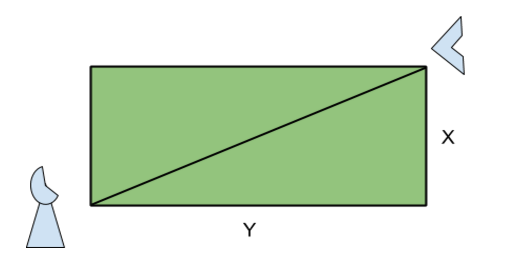
\includegraphics[width=0.8\textwidth]{figures/pic1.png}
  	\caption[Pipeline survey]{Scenario}
\end{figure}

Given the area of the rectangle we can compute the maximum distances of communication, which is the diagonal of the rectangle: 
\begin{equation*}\label{eq:scenario_parameters2} 
 		d_{max} = \sqrt{x^2 + y^2}
\end{equation*}
This distance will be taken into account when computing the radio link communication between the drone and GNS.

\chapter{Hardware setup}\label{ch:hardwaresetup}

\section{Unmanned Aerial System (UAS)}
In some cases it is necessary to talk about our system as a whole, such that we use it further. The UAS can be seen in Figure \ref{fig:uas} and it is composed of the following:
\begin{itemize}
	\item Drone
	\item GNS
	\item Communications
	\item Survey camera
\end{itemize}

\begin{figure}[h]
	\centering
	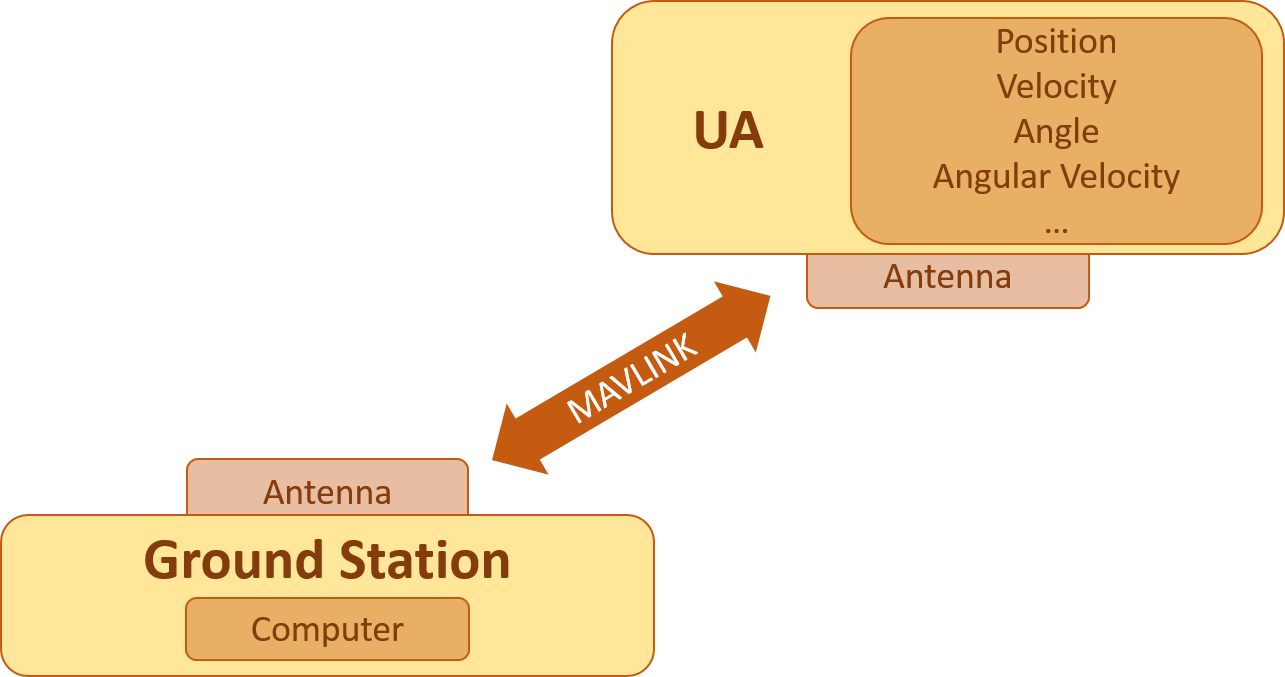
\includegraphics[scale=0.33]{figures/uas.png}
	\caption{Unmanned Aerial System Overview}
	\label{fig:uas}
\end{figure}

In order to have some bounds of the system we can have a look at the drone performances:
\begin{itemize}
	\item 50 km/h - stability at high speeds 
	\item 40 minutes - battery autonomy (30 minutes with payload)
	\item 2400 m - maximum flight altitude (higher if take off from mountain site)
	\item 50 km - maximum radio communication (with directional antennas)
	\item under 1 m - absolute positioning of X-Y GPS
	\item GPS return-to Home (automatically activates when radio link is lost)
\end{itemize}

\subsection{Drone Overview}
			! !	! ! ! ! ! ! ! ! ! ! ! !
! ! ! ! ! ! ! WE NEED SOMETHING HERE ! ! ! ! ! !
			! ! ! ! ! ! ! ! ! ! ! ! ! !

\begin{figure}[hb]
  \centering
  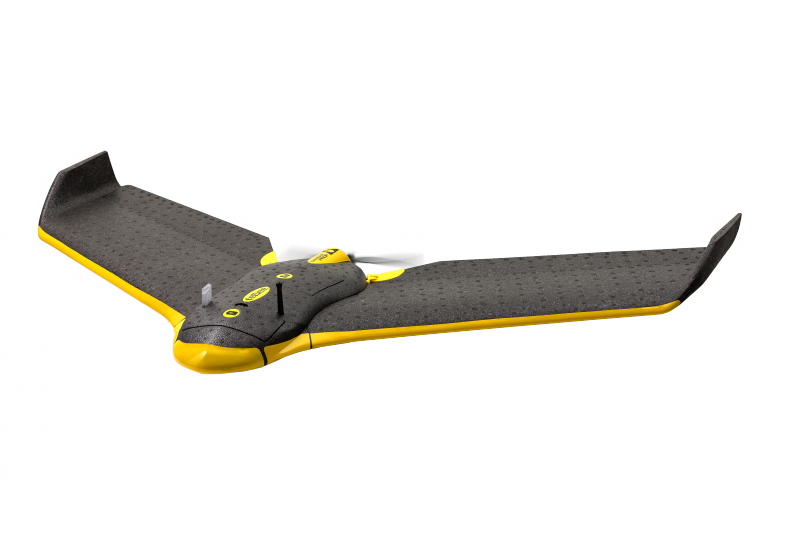
\includegraphics[width=4in]{figures/eBee.png}
  \caption[The professional mapping drone eBee]
   {The professional mapping drone \textit{eBee} \href{https://www.sensefly.com/drones/ebee.html}{(www.sensefly.com)}. Fully autonomous drone to capture high-resolution aerial photos that can transform into accurate 2D orthomosaics \& 3D models.}
\end{figure}

\subsection{GNS Overview}
			! !	! ! ! ! ! ! ! ! ! ! ! !
! ! ! ! ! ! ! WE NEED SOMETHING HERE ! ! ! ! ! !
			! ! ! ! ! ! ! ! ! ! ! ! ! !

\subsection{Antenna Overview}
The antennas used for the GNS and the drone are different by means of weight and size. The preference of using them is based on the application at hand, thus for:
\begin{itemize}
	\item GNS - Parabolic (grid) directional antenna 
	\item Drone - Patch directional antenna
\end{itemize}

A parabolic antenna in an antenna that uses a parabolic reflector and a curved surface to direct the radio waves and its main advantage is that it has a high directivity. This type of antennas are able to produce the narrowest beam widths which allow them to have some of the highest gains.

Parabolic antennas, due to their high gain, are intensively used for carry telephone and television signals between nearby cities. In our specific case, it’s possible to use this property to receive the information provided by the thermal camera through the UAS.

Patch antenna, which is the original type of microstrip, is a low profile antenna that can be mounted on a flat surface and it consists in a rectangular sheet of metal. These antennas are very useful because they are very thin and their directivity varies from 5 to 7 dB.

\begin{table}[h!]
	\centering
	\begin{tabular}{|c||c|c|}
		\hline
		Parameter & GNS & Drone\\ \hline\hline
		Type & Parabolic & Patch\\ \hline
		Polarization & Linear & Linear\\ \hline
		Frequency [GHz] & $2.4$ & $2.4$\\ \hline
		Gain [dB] & $24$ & $14$\\ \hline
		HPBW/$H(^{\circ})$ & $14$ & $45$\\ \hline
		HPBW/$V(^{\circ})$ & $10$ & $45$\\ \hline
	\end{tabular}
	\caption{Table of antennas parameters}
	\label{table:1}
\end{table}

\subsection{Technical Scenario}
As mentioned before we need to assure the maximum distance of communication possible between the GNS and the drone at a certain working frequency:

\begin{equation*}\label{eq:tech_parameters1} 
 	\begin{cases}
 		d_{max} = 50 km	\\
 		f = 2.4 GHz
 	\end{cases}
\end{equation*}

Computing signal wavelength ($\lambda$) for the working frequency stated above:
\begin{equation*}\label{eq:tech_parameters2}
	\lambda = \frac{c}{f} = \frac{3\cdot 10^{8}}{2.4\cdot 10^{9}} 
	        = 0.125 \text{m}
\end{equation*}

Computing the path loss for a distance of 50 kilometers and the signal wavelength:
\begin{equation*}\label{eq:tech_parameters3}
	L = 20\lg\left (\frac{4\pi d_{max}}{\lambda} \right)
	  = 20\lg\left (\frac{4\pi \cdot 50}{0.125\cdot 10^{-3}} \right)
	  = 134 \text{dB} 
\end{equation*}

Computing the output power of the transmitting antenna of 1 Watt:
\begin{equation*}\label{eq:tech_parameters4}
	P_{TX} = 10\lg\left (\frac{1}{10^{-3}} \right)  
	       = 30 \text{dBm}
\end{equation*}


A simplified link budget omitting some losses of the UAS:
\begin{equation*}\label{eq:tech_parameters5}
	P_{RX} = P_{TX} + G_{TX} + G_{RX} - L  
	       = 30 + 24 + 14 - 134 = -66 \text{dBm}
\end{equation*}

\section{Controller system}
\href{http://ctms.engin.umich.edu/CTMS/index.php?example=MotorPosition&section=SystemModeling}{DC Motor Position: System Modeling}

\subsection{Physical setup}
A common actuator in control systems is the DC motor. It directly provides rotary motion and, coupled with wheels or drums and cables, can provide translational motion. The electric equivalent circuit of the armature and the free-body diagram of the rotor are shown in the following figure. 

\begin{figure}[h!]\label{fig:motor_model}
	\centering
	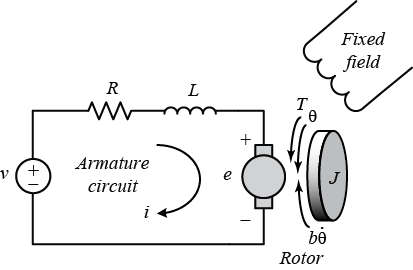
\includegraphics[width=0.7\textwidth]{figures/motor.png}
	\caption{DC Servo Motor}
\end{figure}

From the figure above, we can derive the following governing equations based on Newton's 2nd law and Kirchhoff's voltage law.

\begin{equation}
	J \dot{\dot{\Theta}} + b\dot{\Theta} = Ki \\
	L\frac{di}{dt} + Ri = V - K\dot{\Theta}
\end{equation}

\subsection{Transfer function}
Applying the Laplace transform, the above modeling equations can be expressed in terms of the Laplace variable s. On the link they dont consider initial condition and we want them.

\begin{equation}
	\mathscr{L}\{J \dot{\dot{\Theta}}\}  + \mathscr{L}\{b\dot{\Theta}\} = \mathscr{L}\{Ki\}
\end{equation}

The result become:
\begin{align*}
	& L(I(s)s-i(0)) + RI(s) = V(s) - K(s\Theta (s) - \theta (0)) \\
	& \Rightarrow I(s)(Ls+R) = V(s) - K(s\Theta (s) - \theta (0)) +Li(0) \\
	& \Rightarrow I(s) = \frac{V(s) - K(s\Theta (s) - \theta (0)) +Li(0)}{(Ls+R)}
\end{align*}

Kirchoffs voltage law:
\begin{equation*}
	\mathscr{L}\{L\frac{di}{dt}\} + \mathscr{L}\{Ri\} = \mathscr{L}\{V\} - \mathscr{L}\{K\dot{\Theta}\}
\end{equation*}

The result become:
\begin{align*}
	& J(s^2 \Theta(s) - s\theta (0) - \dot{\theta} (0)) +b(s\Theta (s)-\theta (0)) = KI(s) \\
	& Js^2 J\Theta(s) - Js\theta (0) - J\dot{\theta} (0) +b(s\Theta (s)-\theta (0) = KI(s) 
\end{align*}

And with I(s) inserted:
\begin{align*}
	& Js^2 J\Theta(s) - Js\theta (0) - J\dot{\theta} (0) +b(s\Theta (s)-\theta (0) = K (\frac{V(s) - K(s\Theta (s) - \theta (0)) +Li(0)}{(Ls+R)}) \\
	& (Js^2 J\Theta(s) - Js\theta (0) - J\dot{\theta} (0) +b(s\Theta (s)-\theta (0))(Ls+R) =  K(V(s) - K(s\Theta (s) - \theta (0)) +Li(0)) \\
	& \Theta(s)(Js^2 J +bs) - Js\theta (0) - J\dot{\theta} (0) -\theta (0))(Ls+R) =  K(V(s) - K(s\Theta (s) - \theta (0)) +Li(0))
\end{align*}

And then...
\begin{align*}
	& \Theta(s)((Ls+R)(Js^2 J +bs)+K^2s) + \\
	& (Ls+R)(-Js\theta (0) - J\dot{\theta} (0) -b\theta (0)) = KV(s) - K^2 \theta (0) +KLi(0)
\end{align*}

And then...
\begin{align*}
	\Theta(s) &= \frac{KV(s) - K^2 \theta (0) +KLi(0) - (Ls+R)(-Js\theta (0) - J\dot{\theta} (0) -b\theta (0))}{(Ls+R)(Js^2 J +bs)+K^2s} \\
			  &= \frac{K}{(Ls+R)(Js^2 J +bs)+K^2s}V(s) + \\
	          &\frac{KV(s) - K^2 \theta (0) +KLi(0) - (Ls+R)(-Js\theta (0) - J\dot{\theta} (0) -b\theta (0))}{(Ls+R)(Js^2 J +bs)+K^2s}
\end{align*}

\chapter{Telecommunication}\label{ch:telecommunication}

Drone communication links are generally either radio frequency (RF) or lasercom (optical). Even though both types currently suffer from bandwidth limitations, lasercom could surpass RF in terms of airborne data transfer rate. However, RF will continue to dominate at the lower altitudes for some time into the future because of its better all-weather capability. Additionally, RF links have the advantage of being much more efficient and usually much less complex than lasercom links.
Data rates for RF links have traditionally been restricted due to limited spectrum and
minimization of communication system size, weight, and power.

Radio waves are a form of electromagnetic radiation with frequencies ranging from 3 kHz to 300 GHz. The size and profile constraints of small drones cannot facilitate communication links on the low-frequency (large wavelength) end of the spectrum. 
On the other hand, atmospheric attenuation as well as attenuation by rain, both
exponential in character, becomes a serious limiting factor to the link distance in
the millimeter wavelength region (>300MHz). 
	
Due to these limitations, small drone communication links are restricted to the very high frequency (VHF), the ultrahigh frequency (UHF), and rarely the super-high frequency (SHF) bands.

\section{Telemetry}
One of the main goal of drone surveillance is to procure relevant data. This is done by means of telemetry which is an automated communication process. In this process the data collected is transmitted to a receiving equipment for further processing and monitoring. 

!!! ADD MORE INFO !!!

!!! ADD FIGURE !!!

!!! HOW WE USE IT ? !!!

\section{MAVLink protocol}
When speaking of digital communication it is required to have a certain communication protocol. Given the fact that, this project deals with drones, a special protocol, namely Micro Air Vehicle Link (MAVLink) has been taken into consideration. This protocol is used in a GNS and drones scenario, where inter-communication between systems is needed in order to transmit GPS location, heading angle and speed.  

\subsection{Packet structure}
For further understanding the packet structure of such a protocol is needed as seen in Table \ref{tab:mavlink}.

\begin{table}[h]
	\centering
	\begin{tabular}{|c||c|c|}
		\hline
		Field name       & Index (Bytes)  & Purpose											     \\ \hline\hline
		Start-of-frame   &      0         & Start of frame transmission 							   \\ \hline
		Pay-load-length  &      1         & Length of payload (n)       							   \\ \hline
		Packet sequence  &      2    	  & Sent sequence counter (detect packet loss)                 \\ \hline
		System ID        & 		3		  & Sending system identification 							   \\ \hline
		Component ID     & 		4 		  & Sending component identification 						   \\ \hline
		Message ID       & 		5 		  & Message identification (correctly decoded)      		   \\ \hline
		Payload          &   6 to (n+6)   & Data into the message, depends on Message ID        	   \\ \hline
		CRC              & (n+7) to (n+8) & Check-sum of packet (excluding packet start sign)          \\ \hline
	\end{tabular}
	\caption{MAVLink packet structure}
	\label{tab:mavlink}
\end{table}

The CRC field ensures message integrity of each packet. Another function of the CRC is to establish that both sender and receiver agree on the message transfer. Additionally, a seed value is appended at the end of the data when computing the CRC, generated with every new message.

\subsection{Messages}
As stated above the payload from the packets are MAVLink messages. Also, every message can be identified by its ID field on the packet. Additionally, an XML document (in MAVLink source) has the definition of all the data stored on that payload. A sample of such an XML document can be seen in Figure \ref{fig:mav_msg} which describes a message with an ID 24 giving GPS relevant information.

\begin{figure}[h]
	\centering
	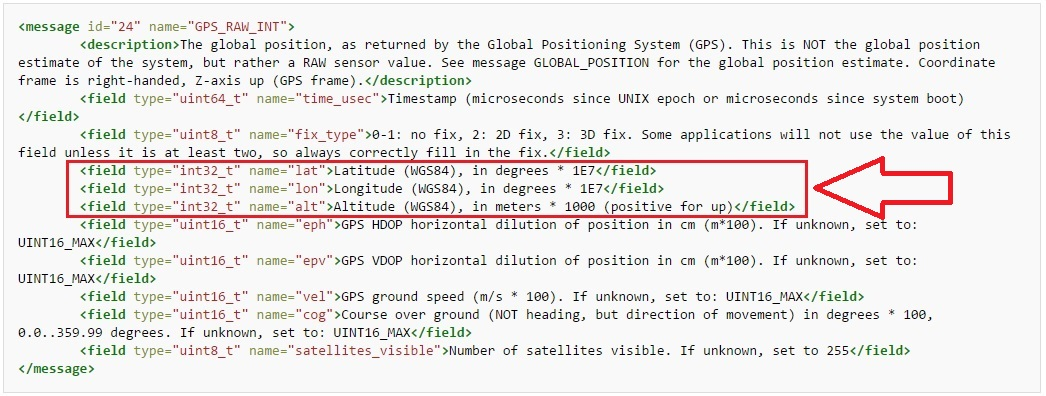
\includegraphics[scale=0.5]{figures/mavlink_msg.jpg}
	\caption{MAVLink message XML document}
	\label{fig:mav_msg}
\end{figure}

To be noted that the XML document describes the logical ordering of the fields for the protocol, not the actual wire format.


\section{Compute Link Budget}

\subsection{Line-Of-Sight Propagation}\label{subsec:los_propagation}
At low frequency (below approximately 3 MHz) radio signals travel as ground waves, which follow the Earth's curvature due to diffraction with the layers of the atmosphere.
However, at higher frequencies and in lower levels of the atmosphere, neither of these effects are significant. Thus any obstruction between the transmitting antenna (transmitter) and the receiving antenna (receiver) will block the signal, just like the light that the eye may sense. Therefore, since the ability to visually see a transmitting antenna (disregarding the limitations of the eye's resolution) roughly corresponds to the ability to receive a radio signal from it, the propagation characteristic of VHF and higher radio frequency (>30 MHz) paths is called line-of-sight. The farthest possible point of propagation is referred to as the radio horizon.

The radio horizon is the locus of points at which direct rays from an antenna are tangential to the surface of the Earth. If the Earth were a perfect sphere and there were no atmosphere, the radio horizon would be a circle.
This way the greatest distance at which a receiver can see the transmitter is explained in the following paragraph.

First, we are going to derive a general expression and after that apply it to a scenario with a drone and a basestation. In figure  \ref{fig:GeometricDist_general} the relationship between the height of the observer above sea level (O point) and the distance d which is between it and the horizon (H point) is shown. Finding this distance is done by the use of the pythagorean theorem. With some simple mathematical calculations the distance d is derived in the following:

\begin{equation}\label{eq:los_distToHorizon}
	(R+h)^2 = R^2+d^2\nonumber \\
	\Rightarrow R^2+2hR+h^2 = R^2+d^2 \Rightarrow d^2 = 2hR + h^2 \\
	\Rightarrow d = \sqrt{2hR + h^2}
\end{equation} 

\begin{figure}
    \hfill
    \subfigure[Geometrical distance to the horizon]{
    	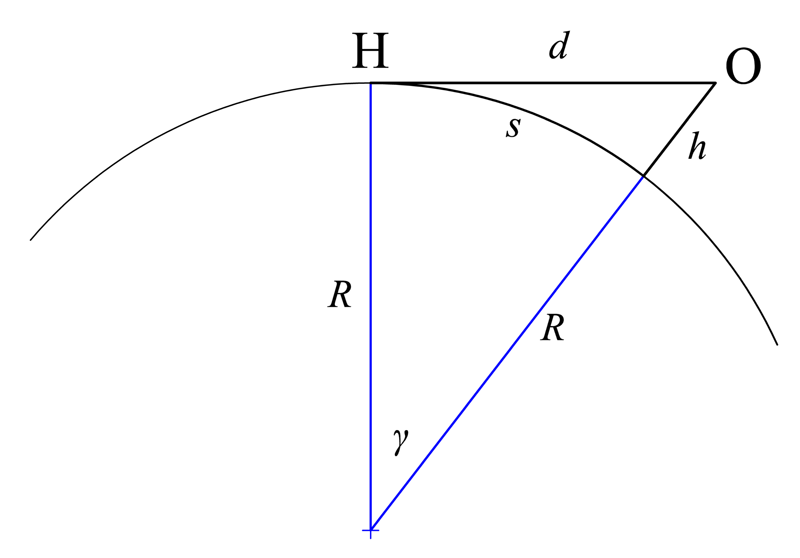
\includegraphics[scale=4]{figures/GeometricDistanceToHorizonOneTriangle.png} 
		\label{fig:GeometricDist_general}}
	\hfill
    \subfigure[Geometrical distance from drone to GNS]{
    	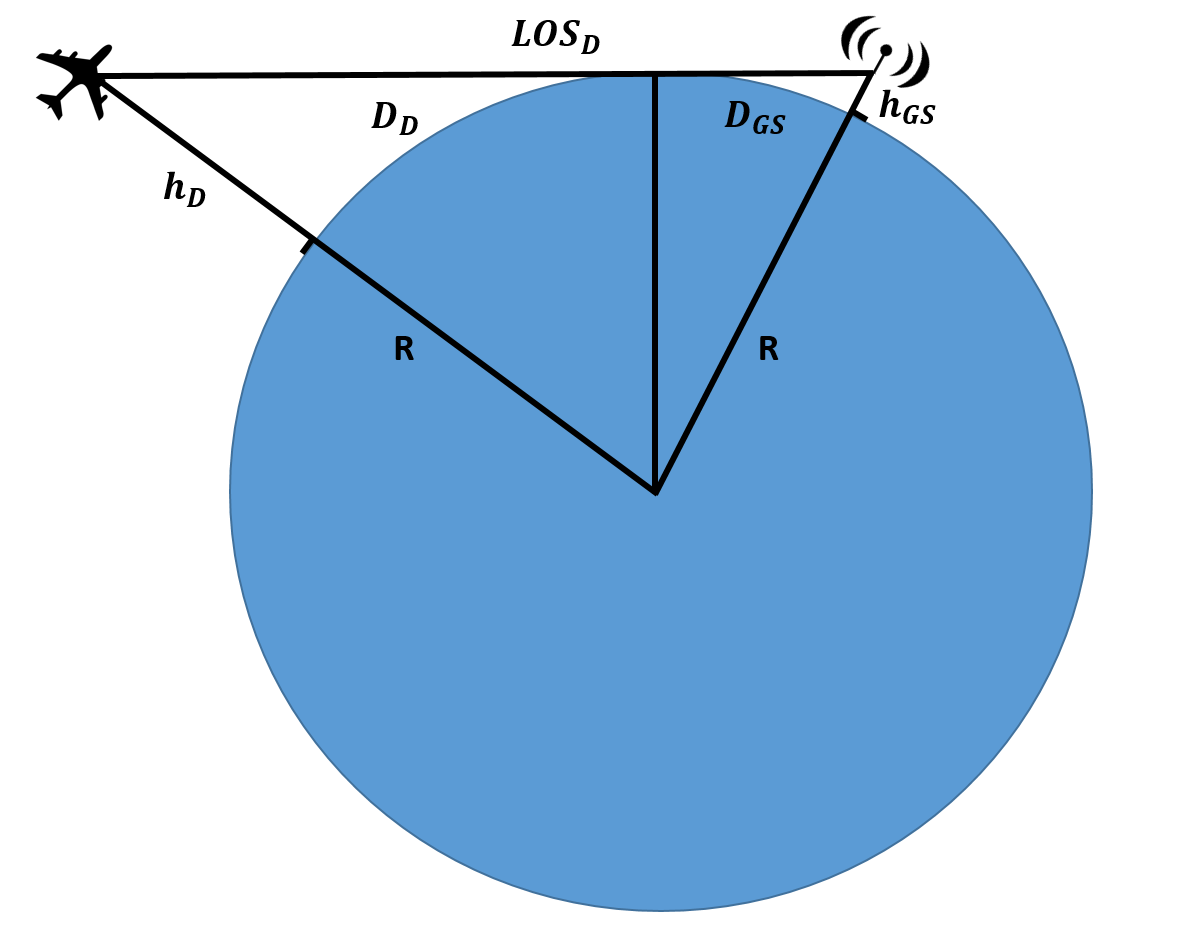
\includegraphics[scale=0.3]{figures/GeometricDistanceToHorizonTwoTriangle.png} 
    	\label{fig:GeometricDist_droneBasestation}}
    \hfill
    \caption{Geometrical distance to the horizon, Pythahorean theorem}
\end{figure}

On figure \ref{fig:GeometricDist_droneBasestation} it is shown that the two objects are a drone and a basestation. Both of them wont be higher then approx 100 meter and since R is radius of the Earth, $2hR$ >> $h^2$ and $h^2$ is therefore neglected in equation \ref{eq:los_distToHorizon}. The two distances $D_D$ and $D_B$ have the same expressions in both cases:
\begin{align*}
	D_D [km] &= \sqrt{2\cdot R \cdot h_D + h_{D}^2} \approx \sqrt{2\cdot 6.378\cdot h_D} = \sqrt{12.756\cdot h_D} = 3.57\cdot \sqrt{h_D} \\
	D_B [km] &= \sqrt{2\cdot R \cdot h_B + h_{B}^2} \approx \sqrt{2\cdot 6.378\cdot h_B} = \sqrt{12.756\cdot h_B} = 3.57\cdot \sqrt{h_B}
\end{align*}

To calculate the distance $D_{DB}$:
\begin{align}
	D_{DB}[km]	 &= D_D + D_B \approx 3.57\cdot \sqrt{h_D} + 3.57\cdot \sqrt{h_B} = {3.57\cdot (\sqrt{h_D} + \sqrt{h_B}} )
\end{align}

\subsection{Example with drone = 100m and basestation = 20m}
Lets take an example if the drone is at $h_D = 100m$ and the basestation at $h_B = 20m$. The distance between the drone and the basestation is as follows:
\begin{equation*}
	D_{DB}[km] = 3.57\cdot (\sqrt{100} + \sqrt{20}) = 51.67km
\end{equation*}

\subsection{Free space path loss}\label{subsec:path_loss}
\paragraph{}
The free space path loss (FSPL) is the loss in signal strength that occurs when an electromagnetic wave travels over a line of sight path in free space. In these circumstances there are no obstacles that might cause the signal to be reflected, refracted, or that might cause additional attenuation. Equation \ref{eq:path_losses} represents the loss in signal strength in dB.

\begin{equation}\label{eq:path_losses}
	L_{FS} = 20\lg\left (\frac{4\pi \cdot d}{\lambda} \right)
\end{equation}

The wave length can also be described by a relationship between the frequency and the velocity of light. This relationship is described by the equation \ref{eq:vel_freq_wavelen1}.

\begin{equation}\label{eq:vel_freq_wavelen1}
	\lambda = \frac{c}{f}
\end{equation}

Explanation of the parameters.
\begin{itemize}
	\item d - distance from transmitter to receiver [m]
	\item $\lambda$ - wavelength of the signal [m]
	\item c - speed of light constant $3\cdot 10^8$ [m/s] 
	\item f - frequency of signal [Hz]
\end{itemize}

Considering our problem we will look into the worst case scenario, which would be maximum distance between the GNS and the drone. 
\begin{equation*}
	Assume 
	\begin{cases}
	d_{max} = \sqrt{x^2+y^2}\\
	\text{f} = f\text{GHz (Should be permitted by law})\\
	\end{cases}
\end{equation*}

Computing signal wavelength:
\begin{equation}\label{eq:vel_freq_wavelen2}
	\lambda = \frac{c}{f} 
	        = \frac{3\cdot 10^{8}}{f\cdot 10^{9}}
	        = \frac{3}{10f}m
\end{equation}

Computing path loss:
\begin{align*}\label{eq:path_loses_calc}
	L = 20\lg\left (\frac{4\pi d}{\lambda} \right) dB 
	 &= 20\lg\left (\frac{4\pi \sqrt{x^2+y^2}}{\frac{3}{10f}} \right) dB\\ 
	 &= 20\lg\left (\frac{4\pi \sqrt{x^2+y^2}\cdot 10f}{ 3} \right) dB
\end{align*}
\noindent \textbf{As an observation, higher distance value between GNS and drone will result in higher path loss.}

\subsection{Link Budget}\label{subsec:link_budget}
\paragraph{}
A link budget is accounting of all of the gains and losses from the transmitter, through the medium  to the receiver in a telecommunication system. It accounts for the attenuation of the transmitted signal due to propagation, as well as the antenna gains, feedline and miscellaneous losses. 
\begin{equation*}\label{eq:link_budget} 
 		\text{Received Power (dBm)} = \text{Transmitted Power (dBm)} + \text{Gains (dB)} - \text{Losses(dB)}
\end{equation*}

In more detailed a common radio link looks like this:

\begin{equation*}\label{eq:link_budget} 
 		P_{RX} = P_{TX} + G_{TX} - L_{TX} - L_{FS} - L_{M} + G_{RX} - L_{RX}
\end{equation*}

Note that decibels are logarithmic measurements, so adding decibels is equivalent to multiplying the actual numeric ratios.


\section{Fresnel zones}
Taking into account that the application at hand involves radio communication it is important to talk about the Fresnel zones. Thus, it can be seen in Figure \ref{fig:fresnel_zones} the three Fresnel zones on the transmission path between A and B. 

\begin{figure}[h]
	\centering
	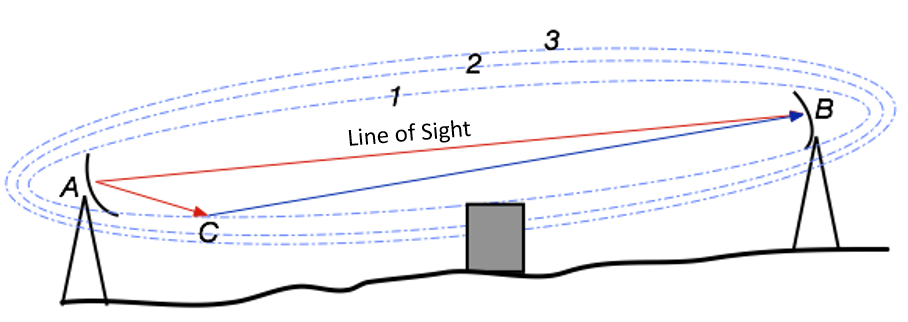
\includegraphics[scale=0.65]{figures/fresnel_zones.png}
	\caption{Fresnel zones between transmitter and receiver}
	\label{fig:fresnel_zones}
\end{figure}


ADD MORE RELEVEANT THINGS 

! ! ! ! \url{https://en.wikipedia.org/wiki/Fresnel_zone}  ! ! ! !


\chapter{Verification}\label{ch:verification}
Our verification.
\subsection{Simulation}

\begin{frame}{Simulation}{LOS Coverage Map}
  \begin{block}{Parameters taken into account for map simulation:}

	  \begin{itemize}
	  	\item Terrain elevation
	  	\item Curvature of the Earth
	  	\item Altitude of UA and GS
	  \end{itemize}

	  \begin{figure}
        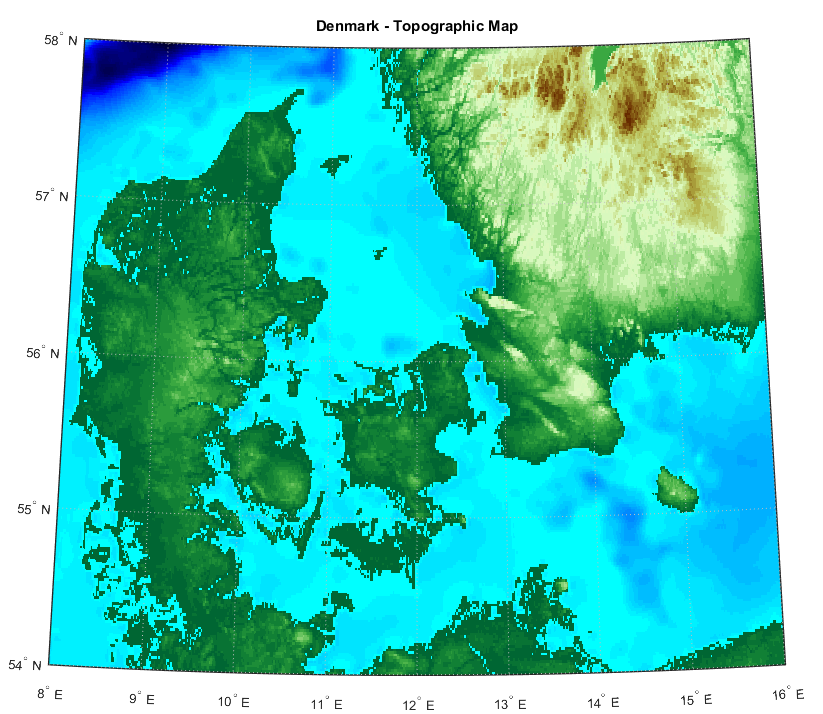
\includegraphics[scale=0.26]{../report/figures/dk_map.png}
      \end{figure}
  
  \end{block}
\end{frame}

\begin{frame}{Simulation}{LOS Coverage Map}
  \begin{block}{Working Principle}
	  \begin{itemize}
	  	\item Import topography map
	  	\item Input GS and UA altitude
	  	\item Choose GS and UA locations on map to plot LOS distance
	  	\item Choose GS location on map to plot LOS coverage map
	  \end{itemize}
  \end{block}
\end{frame}

\begin{frame}{Simulation}{LOS between UA and GS} 
  	\begin{figure}
        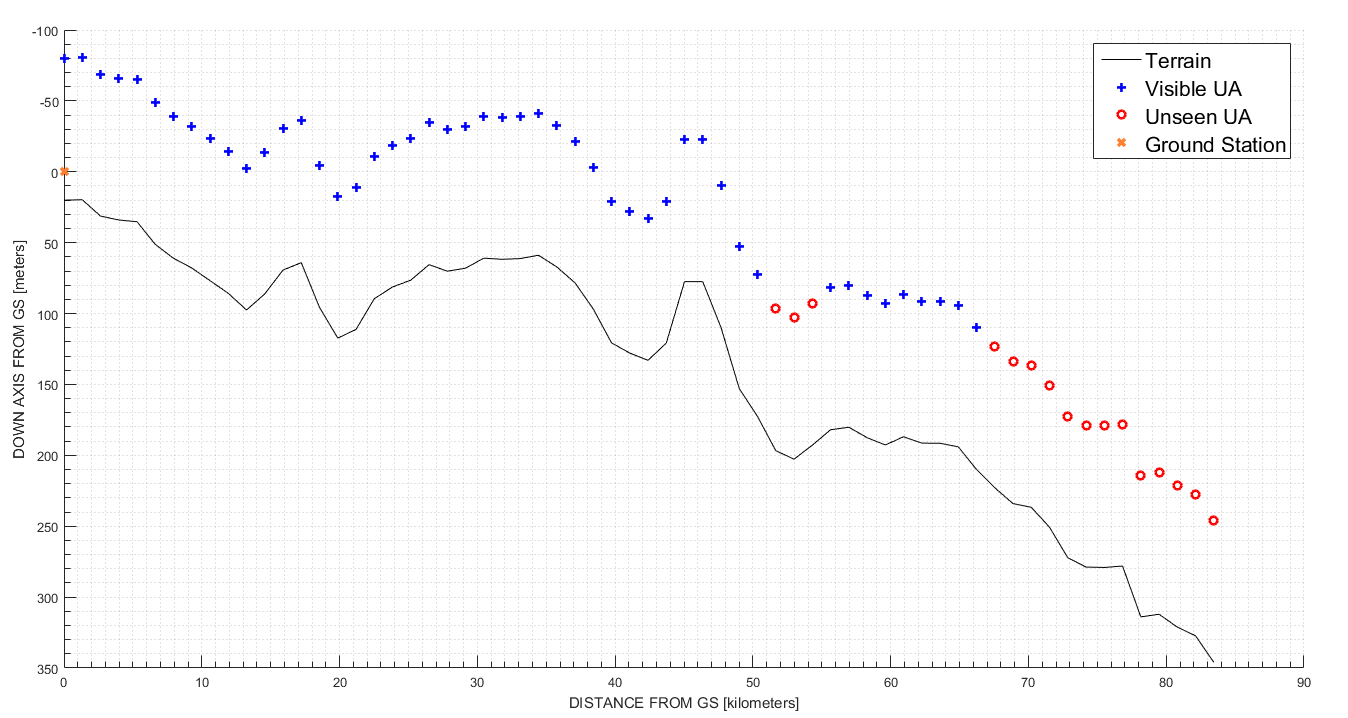
\includegraphics[scale=0.29]{../report/figures/los_2points.png}
    \end{figure}
\end{frame}

\begin{frame}{Simulation}{LOS Coverage Map} 
  	\begin{figure}
        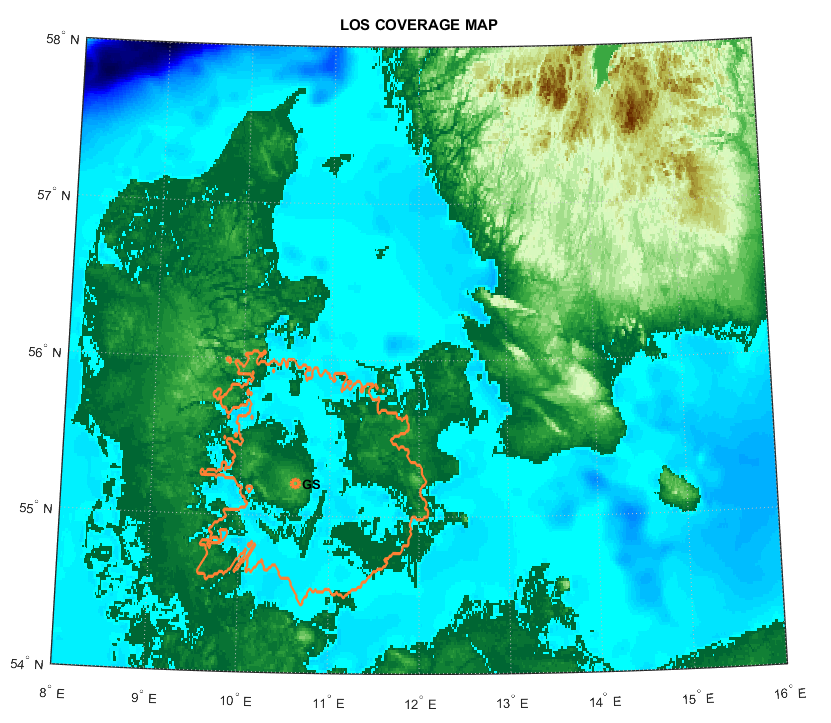
\includegraphics[scale=0.40]{../report/figures/los_odense.png}
    \end{figure}
\end{frame}

\begin{frame}{Simulation}{2D UAS}
	\begin{block}{2D UAS Block Diagram}
		\begin{itemize}
		  	\item Cartesian system (Simplistic)
		  	\item 1 DoF - azimuth angle ($\theta$)
		  	\item Compute optimal azimuth angle for UA and GS 
		\end{itemize}

		\begin{figure}
	        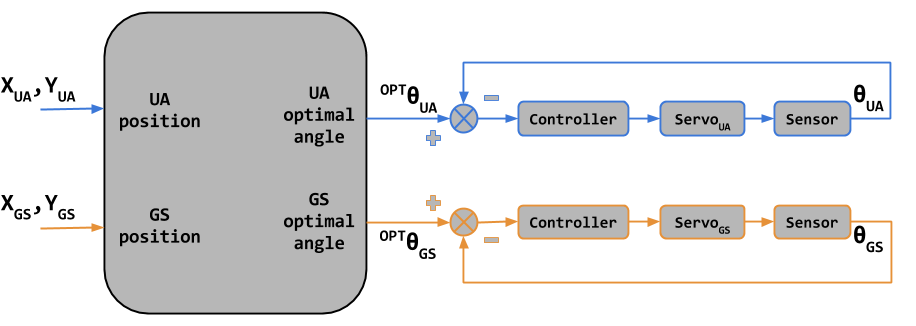
\includegraphics[scale=0.32]{figures/2D_system.png}
	    \end{figure}
    \end{block}
\end{frame}

\begin{frame}{Simulation}{3D UAS}
  \begin{block}{3D UAS Block Diagram}
	\begin{itemize}
	  	\item Realistic Earth Model - WGS84
	  	\item Curvature of the Earth
	  	\item Relief of Earth's surface 
	  	\item Real GPS position: latitude, longitude and altitude
	\end{itemize}

	\begin{figure}
		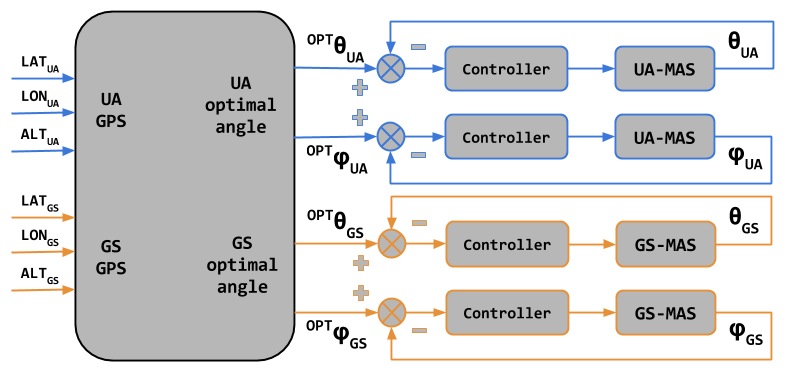
\includegraphics[scale=0.33]{figures/3D_system.png}
	\end{figure}
  \end{block}
\end{frame}

%\chapter{Chapter 2 name}\label{ch:ch2label}
Here is chapter 2. If you want to leearn \todo{I think this word is mispelled} more about \LaTeXe{}, have a look at \cite{Madsen2010}, \cite{Oetiker2010} and \cite{Mittelbach2005}.
\missingfigure{We need a figure right here!}


\chapter{Results and Discussion}\label{ch:results}
Taking into account the 3D simulation discussed in Chapter \ref{ch:sim} 
\chapter{Conclusion}\label{ch:conclusion}
In case you have questions, comments, suggestions or have found a bug, please do not hesitate to contact me. You can find my contact details below.
  \begin{center}
    Jesper Kjær Nielsen\\
    \href{mailto: jkn@es.aau.dk}{jkn@es.aau.dk}\\
    \href{http://kom.aau.dk/~jkn}{http://kom.aau.dk/\textasciitilde jkn}\\
    Fredrik Bajers Vej 7\\
    9220 Aalborg Ø
  \end{center}

\printbibliography[heading=bibintoc]
\label{bib:mybiblio}
%\appendix
%\chapter{Appendix}\label{ch:appAlabel}


\end{document}